\documentclass[x11names]{beamer}
\usepackage{etex,beamerfoils}
\usepackage{array,pifont,amsmath,latexsym,epsfig,amsfonts,yfonts}
\usepackage{amstext,amsopn,amsxtra,amsgen,amsbsy,amscd,amssymb,dcolumn,graphicx}
\usepackage[normalem]{ulem}
\usepackage[all]{xy}
\beamertemplatetheoremsnumbered
\setbeamertemplate{caption}[numbered]
\usetheme{Copenhagen}
\definecolor{NewBlue}{RGB}{4, 114, 155}
\definecolor{magenta}{cmyk}{0,1,0,0}
\usecolortheme[named=NewBlue]{structure}
%\usecolortheme[named=SkyBlue4]{structure}


\newcommand{\comment}[1]{}
\newcommand{\D}{\displaystyle}
\newcommand{\E}{\begin{eqnarray*}}
\newcommand{\F}{\end{eqnarray*}}
\newcommand{\EE}{\begin{eqnarray}}
\newcommand{\FF}{\end{eqnarray}}
\newcommand{\IZ}{\begin{itemize}}
\newcommand{\ZI}{\end{itemize}}
\newcommand{\EN}{\begin{enumerate}}
\newcommand{\NE}{\end{enumerate}}
\newcommand{\itemc}{\item[$\circ$]}
\newcommand{\IZdash}{\begin{itemize} \renewcommand{\labelitemi}{-}}
\newcommand{\tn}{\textnormal}

\newcommand{\itemi}{\item<1->}
\newcommand{\itemii}{\item<2->}
\newcommand{\itemiii}{\item<3->}
\newcommand{\itemiv}{\item<4->}
\newcommand{\itemv}{\item<5->}
\newcommand{\itemvi}{\item<6->}
\newcommand{\itemvii}{\item<7->}
\newcommand{\itemviii}{\item<8->}
\newcommand{\itemix}{\item<9->}
\newcommand{\itemx}{\item<10->}

\newcommand{\itemci}{\item[$\circ$]<1->}
\newcommand{\itemcii}{\item[$\circ$]<2->}
\newcommand{\itemciii}{\item[$\circ$]<3->}
\newcommand{\itemciv}{\item[$\circ$]<4->}
\newcommand{\itemcv}{\item[$\circ$]<5->}
\newcommand{\itemcvi}{\item[$\circ$]<6->}
\newcommand{\itemcvii}{\item[$\circ$]<7->}
\newcommand{\itemcviii}{\item[$\circ$]<8->}
\newcommand{\itemcix}{\item[$\circ$]<9->}
\newcommand{\itemcx}{\item[$\circ$]<10->}

\newcommand{\fr}{\frame}
\newcommand{\ft}{\frametitle}
\newcommand{\ons}{\onslide}
\newcommand{\tc}{\textcolor}

\title[Bank Assets and Liabilities\hspace{2em}\insertframenumber/
\inserttotalframenumber]{Assets and Liabilities of Commercial Banks in the United States}
\author{Brian C.~Jenkins \\ ~ \\University of California, Irvine}

\begin{document}

\frame{\maketitle}


\fr{
\ft{Assets and liabilities of Commercial Banks in the US as of October 10, 2014}
\begin{center}\begin{tabular}{|lp{3cm}c|} \hline && \\ && \textbf{Billions of \$} \\\hline &&\\
\textbf{Assets} &&14,839.5\\&&\\
\textbf{Liabilities} &&13,243.4\\&&\\\hline && \\
\textbf{Capital} &&1,596.1\\&&\\\hline
\end{tabular}\end{center}

\

Source: Data for this table and for subsequent tables and figures obtained from the Federal Reserve Economic Database (FRED) at \href{http://research.stlouisfed.org/fred2/}{http://research.stlouisfed.org/fred2/}.
}
\fr{
\ft{Assets of Commercial Banks in the US as of October 10, 2014}
\begin{tabular}{p{5cm}cc} \hline & \textbf{Billions of \$} & \textbf{Percent of Total}\\\hline\\
\textbf{Loans and Leases} & 7,764.7& 52.3\%\\\\
\textbf{Securities} & 2,834.1& 19.1\%\\\\
\textbf{Loan/Lease Loss Allowance} & -113.5& -0.8\%\\\\
\textbf{Interbank Loans} & 112.4& 0.8\%\\\\
\textbf{Cash Assets} & 2,900.9& 19.5\%\\\\
\textbf{Other Assets} & 1,340.9& 9.0\%\\\\\hline
\textbf{Total Assets} & 14,839.5& 100\%\\\\
\end{tabular}
}
\fr{
\begin{figure}[h] \caption{\label{fig2} \textbf{Assets of Commercial banks in the US from January 1, 1975 through October 10, 2014}}
\hspace*{-.5cm}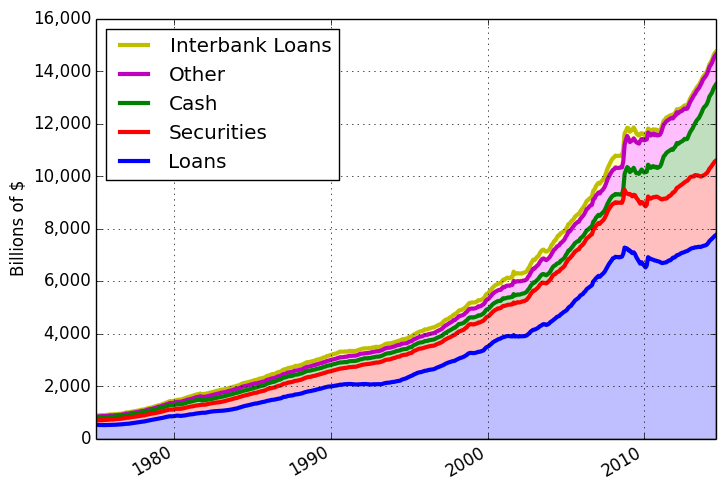
\includegraphics[height = 7.cm]{fig_012_bank_assets.png}
\end{figure}
}
\fr{
\ft{Loans and Leases of Banks in the US as of October 10, 2014}
\begin{tabular}{p{5cm}cc} \hline & \textbf{Billions of \$} & \textbf{Percent of Total}\\\hline\\
\textbf{Commerical/Industrial} & 1,723.5& 22.2\%\\\\
\textbf{Real Estate} & 3,611.7& 46.5\%\\\\
\textbf{Consumer} & 1,181.8& 15.2\%\\\\
\textbf{Other} & 1,247.7& 16.1\%\\\\\hline
\textbf{Total Loans / Leases} & 7,764.7& 100\%\\\\
\end{tabular}
}
\fr{
\ft{Liabilities of Commercial Banks in the US as of October 10, 2014}
\begin{tabular}{p{5cm}cc} \hline & \textbf{Billions of \$} & \textbf{Percent of Total}\\\hline\\
\textbf{Total Deposits} & 10,235.0& 77.3\%\\\\
\textbf{Borrowings} & 1,717.4& 13.0\%\\\\
\textbf{Other Liabilities} & 397.4& 3.0\%\\\\\hline
\textbf{Total Liabilities} & 13,243.4& 100\%\\\\
\end{tabular}
}
\fr{
\begin{figure}[h] \caption{\label{fig2} \textbf{Liabilities of Commercial banks in the US from January 1, 1975 through October 10, 2014}}
\hspace*{-.5cm}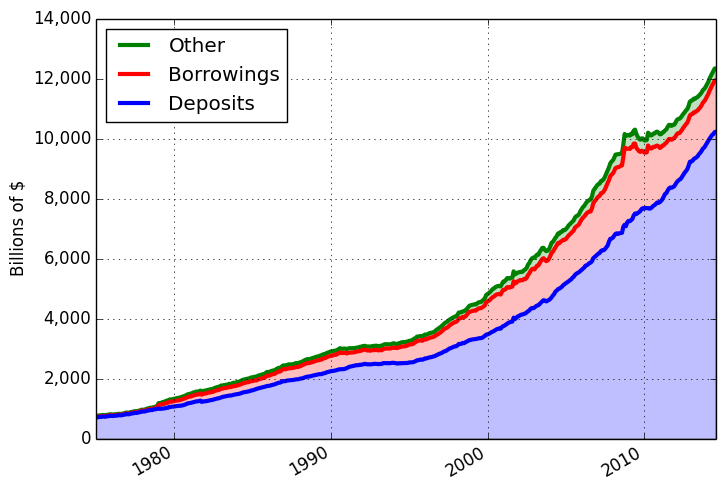
\includegraphics[height = 7.cm]{fig_012_bank_liabilities.png}
\end{figure}
}



\end{document}
